\documentclass[twoside]{book}

% Packages required by doxygen
\usepackage{calc}
\usepackage{doxygen}
\usepackage{graphicx}
\usepackage[utf8]{inputenc}
\usepackage{makeidx}
\usepackage{multicol}
\usepackage{multirow}
\usepackage{textcomp}
\usepackage[table]{xcolor}

% Font selection
\usepackage[T1]{fontenc}
\usepackage{mathptmx}
\usepackage[scaled=.90]{helvet}
\usepackage{courier}
\usepackage{amssymb}
\usepackage{sectsty}
\renewcommand{\familydefault}{\sfdefault}
\allsectionsfont{%
  \fontseries{bc}\selectfont%
  \color{darkgray}%
}
\renewcommand{\DoxyLabelFont}{%
  \fontseries{bc}\selectfont%
  \color{darkgray}%
}

% Page & text layout
\usepackage{geometry}
\geometry{%
  a4paper,%
  top=2.5cm,%
  bottom=2.5cm,%
  left=2.5cm,%
  right=2.5cm%
}
\tolerance=750
\hfuzz=15pt
\hbadness=750
\setlength{\emergencystretch}{15pt}
\setlength{\parindent}{0cm}
\setlength{\parskip}{0.2cm}
\makeatletter
\renewcommand{\paragraph}{%
  \@startsection{paragraph}{4}{0ex}{-1.0ex}{1.0ex}{%
    \normalfont\normalsize\bfseries\SS@parafont%
  }%
}
\renewcommand{\subparagraph}{%
  \@startsection{subparagraph}{5}{0ex}{-1.0ex}{1.0ex}{%
    \normalfont\normalsize\bfseries\SS@subparafont%
  }%
}
\makeatother

% Headers & footers
\usepackage{fancyhdr}
\pagestyle{fancyplain}
\fancyhead[LE]{\fancyplain{}{\bfseries\thepage}}
\fancyhead[CE]{\fancyplain{}{}}
\fancyhead[RE]{\fancyplain{}{\bfseries\leftmark}}
\fancyhead[LO]{\fancyplain{}{\bfseries\rightmark}}
\fancyhead[CO]{\fancyplain{}{}}
\fancyhead[RO]{\fancyplain{}{\bfseries\thepage}}
\fancyfoot[LE]{\fancyplain{}{}}
\fancyfoot[CE]{\fancyplain{}{}}
\fancyfoot[RE]{\fancyplain{}{\bfseries\scriptsize Generated on Wed Apr 20 2016 18\-:34\-:41 for My Project by Doxygen }}
\fancyfoot[LO]{\fancyplain{}{\bfseries\scriptsize Generated on Wed Apr 20 2016 18\-:34\-:41 for My Project by Doxygen }}
\fancyfoot[CO]{\fancyplain{}{}}
\fancyfoot[RO]{\fancyplain{}{}}
\renewcommand{\footrulewidth}{0.4pt}
\renewcommand{\chaptermark}[1]{%
  \markboth{#1}{}%
}
\renewcommand{\sectionmark}[1]{%
  \markright{\thesection\ #1}%
}

% Indices & bibliography
\usepackage{natbib}
\usepackage[titles]{tocloft}
\setcounter{tocdepth}{3}
\setcounter{secnumdepth}{5}
\makeindex

% Hyperlinks (required, but should be loaded last)
\usepackage{ifpdf}
\ifpdf
  \usepackage[pdftex,pagebackref=true]{hyperref}
\else
  \usepackage[ps2pdf,pagebackref=true]{hyperref}
\fi
\hypersetup{%
  colorlinks=true,%
  linkcolor=blue,%
  citecolor=blue,%
  unicode%
}

% Custom commands
\newcommand{\clearemptydoublepage}{%
  \newpage{\pagestyle{empty}\cleardoublepage}%
}


%===== C O N T E N T S =====

\begin{document}

% Titlepage & ToC
\hypersetup{pageanchor=false}
\pagenumbering{roman}
\begin{titlepage}
\vspace*{7cm}
\begin{center}%
{\Large My Project }\\
\vspace*{1cm}
{\large Generated by Doxygen 1.8.6}\\
\vspace*{0.5cm}
{\small Wed Apr 20 2016 18:34:41}\\
\end{center}
\end{titlepage}
\clearemptydoublepage
\tableofcontents
\clearemptydoublepage
\pagenumbering{arabic}
\hypersetup{pageanchor=true}

%--- Begin generated contents ---
\chapter{O\-O\-P-\/polygons}
\label{md_README}
\hypertarget{md_README}{}
A repository for my O\-O\-P in C++ project for The University of Manchester.

Project brief\-: \char`\"{}\-Design a class hierarchy for creating and manipulating polygon shapes, storing the vector co-\/ordinates of each vertex\char`\"{} 
\chapter{Hierarchical Index}
\section{Class Hierarchy}
This inheritance list is sorted roughly, but not completely, alphabetically\-:\begin{DoxyCompactList}
\item \contentsline{section}{polygons\-:\-:app$<$ T $>$}{\pageref{classpolygons_1_1app}}{}
\item \contentsline{section}{polygons\-:\-:manager$<$ T $>$}{\pageref{classpolygons_1_1manager}}{}
\item \contentsline{section}{polygons\-:\-:polygon$<$ T $>$}{\pageref{classpolygons_1_1polygon}}{}
\begin{DoxyCompactList}
\item \contentsline{section}{polygons\-:\-:equi\-Triangle$<$ T $>$}{\pageref{classpolygons_1_1equiTriangle}}{}
\begin{DoxyCompactList}
\item \contentsline{section}{polygons\-:\-:iso\-Triangle$<$ T $>$}{\pageref{classpolygons_1_1isoTriangle}}{}
\end{DoxyCompactList}
\item \contentsline{section}{polygons\-:\-:hexagon$<$ T $>$}{\pageref{classpolygons_1_1hexagon}}{}
\item \contentsline{section}{polygons\-:\-:pentagon$<$ T $>$}{\pageref{classpolygons_1_1pentagon}}{}
\item \contentsline{section}{polygons\-:\-:square$<$ T $>$}{\pageref{classpolygons_1_1square}}{}
\begin{DoxyCompactList}
\item \contentsline{section}{polygons\-:\-:rectangle$<$ T $>$}{\pageref{classpolygons_1_1rectangle}}{}
\end{DoxyCompactList}
\end{DoxyCompactList}
\item \contentsline{section}{polygons\-:\-:vertex$<$ T $>$}{\pageref{classpolygons_1_1vertex}}{}
\end{DoxyCompactList}

\chapter{Class Index}
\section{Class List}
Here are the classes, structs, unions and interfaces with brief descriptions\-:\begin{DoxyCompactList}
\item\contentsline{section}{\hyperlink{classpolygons_1_1app}{polygons\-::app$<$ T $>$} }{\pageref{classpolygons_1_1app}}{}
\item\contentsline{section}{\hyperlink{classpolygons_1_1equiTriangle}{polygons\-::equi\-Triangle$<$ T $>$} }{\pageref{classpolygons_1_1equiTriangle}}{}
\item\contentsline{section}{\hyperlink{classpolygons_1_1hexagon}{polygons\-::hexagon$<$ T $>$} }{\pageref{classpolygons_1_1hexagon}}{}
\item\contentsline{section}{\hyperlink{classpolygons_1_1isoTriangle}{polygons\-::iso\-Triangle$<$ T $>$} }{\pageref{classpolygons_1_1isoTriangle}}{}
\item\contentsline{section}{\hyperlink{classpolygons_1_1manager}{polygons\-::manager$<$ T $>$} }{\pageref{classpolygons_1_1manager}}{}
\item\contentsline{section}{\hyperlink{classpolygons_1_1pentagon}{polygons\-::pentagon$<$ T $>$} }{\pageref{classpolygons_1_1pentagon}}{}
\item\contentsline{section}{\hyperlink{classpolygons_1_1polygon}{polygons\-::polygon$<$ T $>$} }{\pageref{classpolygons_1_1polygon}}{}
\item\contentsline{section}{\hyperlink{classpolygons_1_1rectangle}{polygons\-::rectangle$<$ T $>$} }{\pageref{classpolygons_1_1rectangle}}{}
\item\contentsline{section}{\hyperlink{classpolygons_1_1square}{polygons\-::square$<$ T $>$} }{\pageref{classpolygons_1_1square}}{}
\item\contentsline{section}{\hyperlink{classpolygons_1_1vertex}{polygons\-::vertex$<$ T $>$} }{\pageref{classpolygons_1_1vertex}}{}
\end{DoxyCompactList}

\chapter{Class Documentation}
\hypertarget{classpolygons_1_1app}{\section{polygons\-:\-:app$<$ T $>$ Class Template Reference}
\label{classpolygons_1_1app}\index{polygons\-::app$<$ T $>$@{polygons\-::app$<$ T $>$}}
}


{\ttfamily \#include $<$app.\-h$>$}

\subsection*{Public Member Functions}
\begin{DoxyCompactItemize}
\item 
\hypertarget{classpolygons_1_1app_aff6d276cee6e502fa086aeb1ce4ad2f8}{{\bfseries app} (\hyperlink{classpolygons_1_1manager}{manager}$<$ T $>$ p\-\_\-man)}\label{classpolygons_1_1app_aff6d276cee6e502fa086aeb1ce4ad2f8}

\item 
\hypertarget{classpolygons_1_1app_ae88f2d95274e77881443122ca42a1cd0}{void {\bfseries start} ()}\label{classpolygons_1_1app_ae88f2d95274e77881443122ca42a1cd0}

\item 
\hypertarget{classpolygons_1_1app_a6d7381dafd5d79a0b8f8a945601521f9}{void {\bfseries end} ()}\label{classpolygons_1_1app_a6d7381dafd5d79a0b8f8a945601521f9}

\end{DoxyCompactItemize}
\subsection*{Protected Member Functions}
\begin{DoxyCompactItemize}
\item 
\hypertarget{classpolygons_1_1app_ad8953bfb86943eb52851971a786d0bf8}{void {\bfseries loop} ()}\label{classpolygons_1_1app_ad8953bfb86943eb52851971a786d0bf8}

\item 
\hypertarget{classpolygons_1_1app_a54b9b363ea71f6a0df9936a5498e05d5}{string {\bfseries get\-New\-Name} ()}\label{classpolygons_1_1app_a54b9b363ea71f6a0df9936a5498e05d5}

\item 
\hypertarget{classpolygons_1_1app_a685b0431705cfa698fbcf15112694a36}{string {\bfseries get\-Existing\-Name} ()}\label{classpolygons_1_1app_a685b0431705cfa698fbcf15112694a36}

\item 
\hypertarget{classpolygons_1_1app_a4f9da856aa9944fa104fd63ff86feb40}{T {\bfseries get\-Number} (bool p\-\_\-positive\-Definite, string p\-\_\-msg)}\label{classpolygons_1_1app_a4f9da856aa9944fa104fd63ff86feb40}

\item 
\hypertarget{classpolygons_1_1app_ab7bed478ee5edd256e1bc6c5ecb34fc1}{string {\bfseries get\-Filename} ()}\label{classpolygons_1_1app_ab7bed478ee5edd256e1bc6c5ecb34fc1}

\item 
\hypertarget{classpolygons_1_1app_a2e559bc56e3dc8aecc344ddfe6a15388}{{\footnotesize template$<$class U $>$ }\\char {\bfseries get\-Option} (initializer\-\_\-list$<$ U $>$ p\-\_\-chars, string p\-\_\-msg)}\label{classpolygons_1_1app_a2e559bc56e3dc8aecc344ddfe6a15388}

\end{DoxyCompactItemize}
\subsection*{Protected Attributes}
\begin{DoxyCompactItemize}
\item 
\hypertarget{classpolygons_1_1app_a9a23bbc7fcd63799c4519c13616285f7}{\hyperlink{classpolygons_1_1manager}{manager}$<$ T $>$ {\bfseries m\-\_\-man}}\label{classpolygons_1_1app_a9a23bbc7fcd63799c4519c13616285f7}

\item 
\hypertarget{classpolygons_1_1app_a0ed33f611d56816f2cad442968e73c8b}{string {\bfseries m\-\_\-file\-Name}}\label{classpolygons_1_1app_a0ed33f611d56816f2cad442968e73c8b}

\item 
\hypertarget{classpolygons_1_1app_a19a74b237359a316270424bac4a82065}{bool {\bfseries m\-\_\-using}}\label{classpolygons_1_1app_a19a74b237359a316270424bac4a82065}

\end{DoxyCompactItemize}


\subsection{Detailed Description}
\subsubsection*{template$<$class T$>$class polygons\-::app$<$ T $>$}

This is a cool comment about the app class 

The documentation for this class was generated from the following file\-:\begin{DoxyCompactItemize}
\item 
app.\-h\end{DoxyCompactItemize}

\hypertarget{classpolygons_1_1equiTriangle}{\section{polygons\-:\-:equi\-Triangle$<$ T $>$ Class Template Reference}
\label{classpolygons_1_1equiTriangle}\index{polygons\-::equi\-Triangle$<$ T $>$@{polygons\-::equi\-Triangle$<$ T $>$}}
}
Inheritance diagram for polygons\-:\-:equi\-Triangle$<$ T $>$\-:\begin{figure}[H]
\begin{center}
\leavevmode
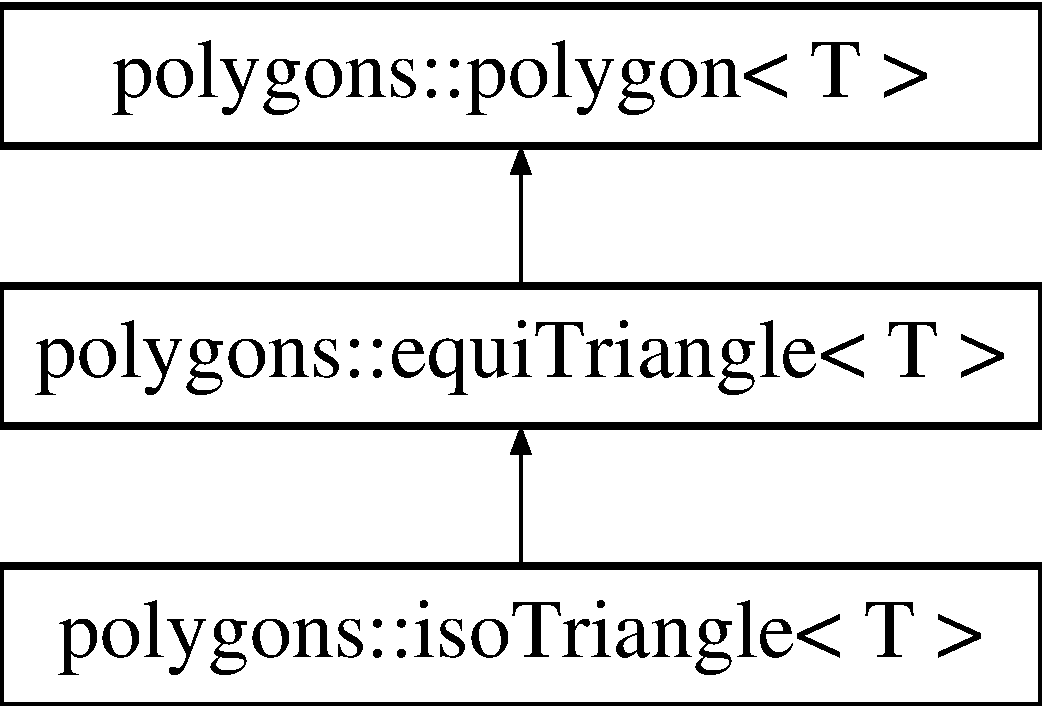
\includegraphics[height=3.000000cm]{classpolygons_1_1equiTriangle}
\end{center}
\end{figure}
\subsection*{Public Member Functions}
\begin{DoxyCompactItemize}
\item 
\hypertarget{classpolygons_1_1equiTriangle_aa8d3b57db828513bc5ea9a9cf58b9672}{{\bfseries equi\-Triangle} (T p\-\_\-x, T p\-\_\-y, T p\-\_\-\-L)}\label{classpolygons_1_1equiTriangle_aa8d3b57db828513bc5ea9a9cf58b9672}

\item 
\hypertarget{classpolygons_1_1equiTriangle_a21f03ae2760d975fb2411355740abdaf}{string {\bfseries type} ()}\label{classpolygons_1_1equiTriangle_a21f03ae2760d975fb2411355740abdaf}

\end{DoxyCompactItemize}
\subsection*{Additional Inherited Members}


The documentation for this class was generated from the following file\-:\begin{DoxyCompactItemize}
\item 
polygon.\-h\end{DoxyCompactItemize}

\hypertarget{classpolygons_1_1hexagon}{\section{polygons\-:\-:hexagon$<$ T $>$ Class Template Reference}
\label{classpolygons_1_1hexagon}\index{polygons\-::hexagon$<$ T $>$@{polygons\-::hexagon$<$ T $>$}}
}
Inheritance diagram for polygons\-:\-:hexagon$<$ T $>$\-:\begin{figure}[H]
\begin{center}
\leavevmode
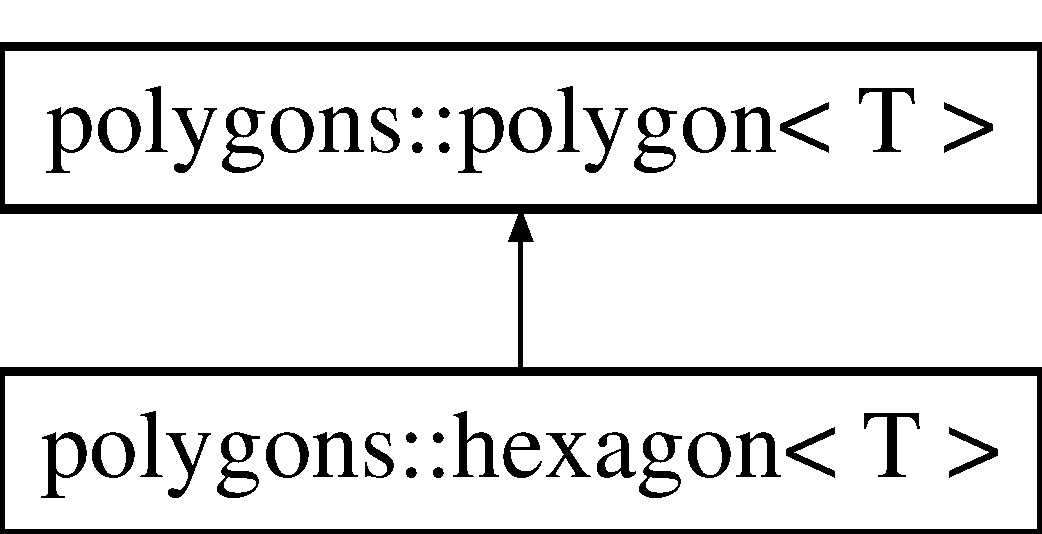
\includegraphics[height=2.000000cm]{classpolygons_1_1hexagon}
\end{center}
\end{figure}
\subsection*{Public Member Functions}
\begin{DoxyCompactItemize}
\item 
\hypertarget{classpolygons_1_1hexagon_a3eca4db8c87b57820f0356943deadad4}{{\bfseries hexagon} (T p\-\_\-x, T p\-\_\-y, T p\-\_\-\-L)}\label{classpolygons_1_1hexagon_a3eca4db8c87b57820f0356943deadad4}

\item 
\hypertarget{classpolygons_1_1hexagon_a7e99cf11e5f1d3c0bfcd612ff238e4b6}{string {\bfseries type} ()}\label{classpolygons_1_1hexagon_a7e99cf11e5f1d3c0bfcd612ff238e4b6}

\end{DoxyCompactItemize}
\subsection*{Additional Inherited Members}


The documentation for this class was generated from the following file\-:\begin{DoxyCompactItemize}
\item 
polygon.\-h\end{DoxyCompactItemize}

\hypertarget{classpolygons_1_1isoTriangle}{\section{polygons\-:\-:iso\-Triangle$<$ T $>$ Class Template Reference}
\label{classpolygons_1_1isoTriangle}\index{polygons\-::iso\-Triangle$<$ T $>$@{polygons\-::iso\-Triangle$<$ T $>$}}
}
Inheritance diagram for polygons\-:\-:iso\-Triangle$<$ T $>$\-:\begin{figure}[H]
\begin{center}
\leavevmode
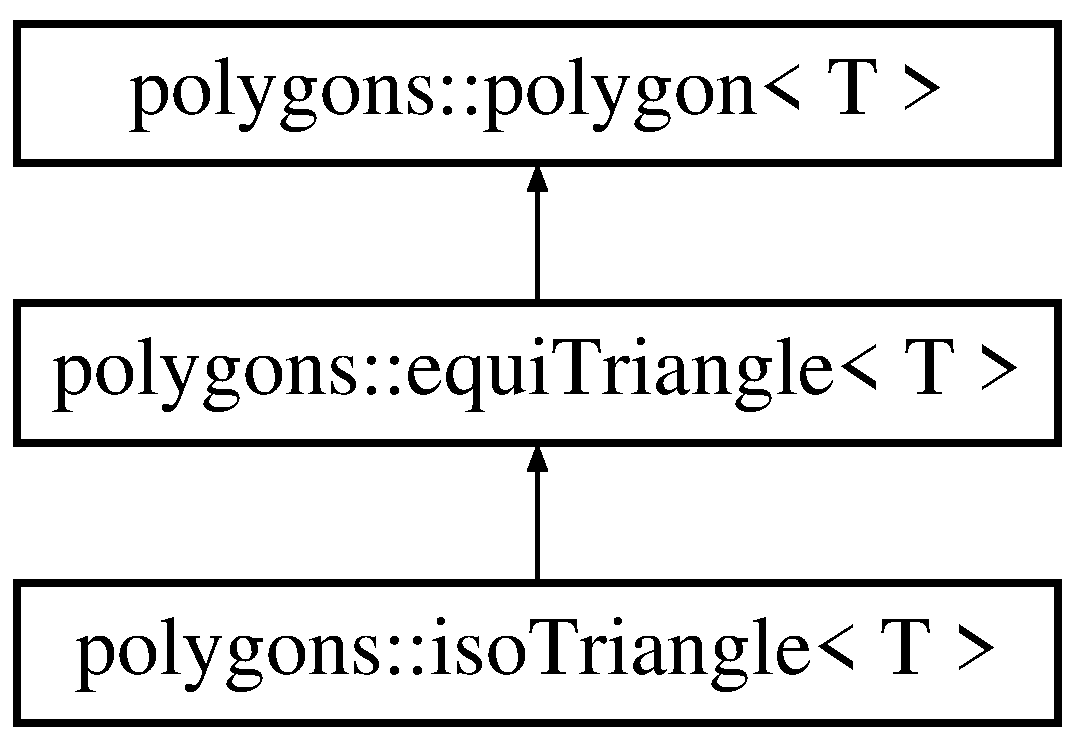
\includegraphics[height=3.000000cm]{classpolygons_1_1isoTriangle}
\end{center}
\end{figure}
\subsection*{Public Member Functions}
\begin{DoxyCompactItemize}
\item 
\hypertarget{classpolygons_1_1isoTriangle_ac6bd6175e17aeb0fdefb661e41425f84}{{\bfseries iso\-Triangle} (T p\-\_\-x, T p\-\_\-y, T p\-\_\-\-B, T p\-\_\-\-L)}\label{classpolygons_1_1isoTriangle_ac6bd6175e17aeb0fdefb661e41425f84}

\item 
\hypertarget{classpolygons_1_1isoTriangle_adf469b12fabb63a710c8e77be5945ccc}{string {\bfseries type} ()}\label{classpolygons_1_1isoTriangle_adf469b12fabb63a710c8e77be5945ccc}

\end{DoxyCompactItemize}
\subsection*{Additional Inherited Members}


The documentation for this class was generated from the following file\-:\begin{DoxyCompactItemize}
\item 
polygon.\-h\end{DoxyCompactItemize}

\hypertarget{classpolygons_1_1manager}{\section{polygons\-:\-:manager$<$ T $>$ Class Template Reference}
\label{classpolygons_1_1manager}\index{polygons\-::manager$<$ T $>$@{polygons\-::manager$<$ T $>$}}
}
\subsection*{Public Member Functions}
\begin{DoxyCompactItemize}
\item 
\hypertarget{classpolygons_1_1manager_a78d63452e32a64e5796b51a08f5b2b68}{void {\bfseries add} (\hyperlink{classpolygons_1_1polygon}{polygon}$<$ T $>$ $\ast$p\-\_\-polygon, string p\-\_\-name)}\label{classpolygons_1_1manager_a78d63452e32a64e5796b51a08f5b2b68}

\item 
\hypertarget{classpolygons_1_1manager_ac1f2398e33cc6ca111edd542fce62f70}{bool {\bfseries exists} (string p\-\_\-name)}\label{classpolygons_1_1manager_ac1f2398e33cc6ca111edd542fce62f70}

\item 
\hypertarget{classpolygons_1_1manager_ae9ed98c7b184436a64ba8a3c837023af}{\hyperlink{classpolygons_1_1polygon}{polygon}$<$ T $>$ $\ast$\& {\bfseries get} (string p\-\_\-name)}\label{classpolygons_1_1manager_ae9ed98c7b184436a64ba8a3c837023af}

\item 
\hypertarget{classpolygons_1_1manager_a0f18da8804c0314a8b7be0737324b14b}{void {\bfseries remove} (string p\-\_\-name)}\label{classpolygons_1_1manager_a0f18da8804c0314a8b7be0737324b14b}

\item 
\hypertarget{classpolygons_1_1manager_a36fb469747b78c08c02e762b7a97e7fb}{void {\bfseries list\-All} ()}\label{classpolygons_1_1manager_a36fb469747b78c08c02e762b7a97e7fb}

\item 
\hypertarget{classpolygons_1_1manager_a9eb125d146b0918f6be7a9906a12f5f6}{void {\bfseries display} (string p\-\_\-filename)}\label{classpolygons_1_1manager_a9eb125d146b0918f6be7a9906a12f5f6}

\item 
\hypertarget{classpolygons_1_1manager_aaeda64d252e495c66322fcb08bb428d0}{int {\bfseries N} ()}\label{classpolygons_1_1manager_aaeda64d252e495c66322fcb08bb428d0}

\end{DoxyCompactItemize}
\subsection*{Protected Attributes}
\begin{DoxyCompactItemize}
\item 
\hypertarget{classpolygons_1_1manager_a4c56d352b76872309478d426ea415d25}{map$<$ string, \hyperlink{classpolygons_1_1polygon}{polygon}$<$ T $>$ $\ast$ $>$ {\bfseries m\-\_\-library}}\label{classpolygons_1_1manager_a4c56d352b76872309478d426ea415d25}

\end{DoxyCompactItemize}


The documentation for this class was generated from the following file\-:\begin{DoxyCompactItemize}
\item 
manager.\-h\end{DoxyCompactItemize}

\hypertarget{classpolygons_1_1pentagon}{\section{polygons\-:\-:pentagon$<$ T $>$ Class Template Reference}
\label{classpolygons_1_1pentagon}\index{polygons\-::pentagon$<$ T $>$@{polygons\-::pentagon$<$ T $>$}}
}
Inheritance diagram for polygons\-:\-:pentagon$<$ T $>$\-:\begin{figure}[H]
\begin{center}
\leavevmode
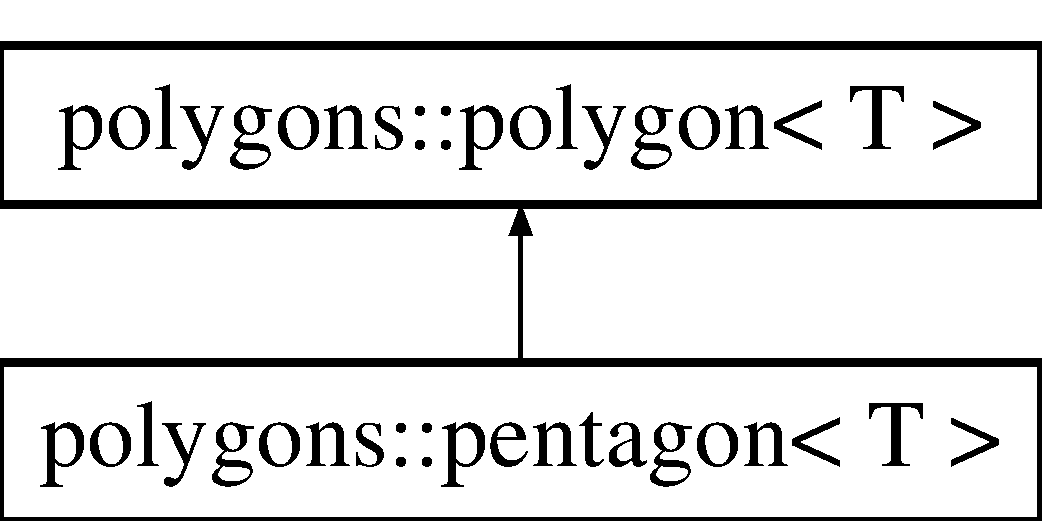
\includegraphics[height=2.000000cm]{classpolygons_1_1pentagon}
\end{center}
\end{figure}
\subsection*{Public Member Functions}
\begin{DoxyCompactItemize}
\item 
\hypertarget{classpolygons_1_1pentagon_a2b36bfb6a6cca42632ca15382c246766}{{\bfseries pentagon} (T p\-\_\-x, T p\-\_\-y, T p\-\_\-\-L)}\label{classpolygons_1_1pentagon_a2b36bfb6a6cca42632ca15382c246766}

\item 
\hypertarget{classpolygons_1_1pentagon_a9c3f3cec5d2116ca493ba2bbf53d778d}{string {\bfseries type} ()}\label{classpolygons_1_1pentagon_a9c3f3cec5d2116ca493ba2bbf53d778d}

\end{DoxyCompactItemize}
\subsection*{Additional Inherited Members}


The documentation for this class was generated from the following file\-:\begin{DoxyCompactItemize}
\item 
polygon.\-h\end{DoxyCompactItemize}

\hypertarget{classpolygons_1_1polygon}{\section{polygons\-:\-:polygon$<$ T $>$ Class Template Reference}
\label{classpolygons_1_1polygon}\index{polygons\-::polygon$<$ T $>$@{polygons\-::polygon$<$ T $>$}}
}
Inheritance diagram for polygons\-:\-:polygon$<$ T $>$\-:\begin{figure}[H]
\begin{center}
\leavevmode
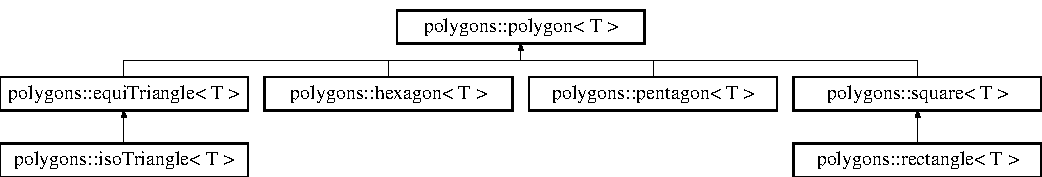
\includegraphics[height=2.372881cm]{classpolygons_1_1polygon}
\end{center}
\end{figure}
\subsection*{Public Member Functions}
\begin{DoxyCompactItemize}
\item 
\hypertarget{classpolygons_1_1polygon_a15af5594d92579ffd4ae2fb51edc3de7}{{\bfseries polygon} (int p\-\_\-\-N, T p\-\_\-x, T p\-\_\-y, T p\-\_\-\-L)}\label{classpolygons_1_1polygon_a15af5594d92579ffd4ae2fb51edc3de7}

\item 
\hypertarget{classpolygons_1_1polygon_a93e192db67d4b8a841066c09838d377a}{{\footnotesize template$<$class U $>$ }\\{\bfseries polygon} (initializer\-\_\-list$<$ U $>$ li)}\label{classpolygons_1_1polygon_a93e192db67d4b8a841066c09838d377a}

\item 
\hypertarget{classpolygons_1_1polygon_a89546d086da3c7b779f3cfac3e17ca47}{int {\bfseries N} ()}\label{classpolygons_1_1polygon_a89546d086da3c7b779f3cfac3e17ca47}

\item 
\hypertarget{classpolygons_1_1polygon_afac16ab826161151ec6c72d76b30963d}{\hyperlink{classpolygons_1_1vertex}{vertex}$<$ T $>$ {\bfseries centre} ()}\label{classpolygons_1_1polygon_afac16ab826161151ec6c72d76b30963d}

\item 
\hypertarget{classpolygons_1_1polygon_a25500df92a688cf99f061bbef709ad14}{\hyperlink{classpolygons_1_1vertex}{vertex}$<$ T $>$ {\bfseries normal} ()}\label{classpolygons_1_1polygon_a25500df92a688cf99f061bbef709ad14}

\item 
\hypertarget{classpolygons_1_1polygon_af26febef898801a19a9d6ddbbde4e4cf}{bool {\bfseries modified} ()}\label{classpolygons_1_1polygon_af26febef898801a19a9d6ddbbde4e4cf}

\item 
\hypertarget{classpolygons_1_1polygon_a3291384abefa6279f035f412f9d0dec3}{virtual string {\bfseries type} ()=0}\label{classpolygons_1_1polygon_a3291384abefa6279f035f412f9d0dec3}

\item 
\hypertarget{classpolygons_1_1polygon_aef5db913d4250fbda4cc40184858c4c1}{void {\bfseries list\-Vertices} ()}\label{classpolygons_1_1polygon_aef5db913d4250fbda4cc40184858c4c1}

\item 
\hypertarget{classpolygons_1_1polygon_a513f206b17fd9a8409e07b4c4a93ce51}{const \hyperlink{classpolygons_1_1vertex}{vertex}$<$ T $>$ \& {\bfseries operator\mbox{[}$\,$\mbox{]}} (int p\-\_\-i)}\label{classpolygons_1_1polygon_a513f206b17fd9a8409e07b4c4a93ce51}

\item 
\hypertarget{classpolygons_1_1polygon_a58b903988793c71055bc2177872164d3}{void {\bfseries translate} (T p\-\_\-x, T p\-\_\-y, T p\-\_\-z)}\label{classpolygons_1_1polygon_a58b903988793c71055bc2177872164d3}

\item 
\hypertarget{classpolygons_1_1polygon_aac0acb96427b60ed992c4d018e972cd5}{void {\bfseries scale} (T p\-\_\-x, T p\-\_\-y, T p\-\_\-z, T p\-\_\-fx, T p\-\_\-fy, T p\-\_\-fz)}\label{classpolygons_1_1polygon_aac0acb96427b60ed992c4d018e972cd5}

\item 
\hypertarget{classpolygons_1_1polygon_a7c9f38badf1fbbbdf3cc8529e039b395}{void {\bfseries scale\-Centre} (T p\-\_\-fx, T p\-\_\-fy, T p\-\_\-fz)}\label{classpolygons_1_1polygon_a7c9f38badf1fbbbdf3cc8529e039b395}

\item 
\hypertarget{classpolygons_1_1polygon_a14a41d7b439f852007a1d82eff7bdb50}{void {\bfseries rotate} (T p\-\_\-x1, T p\-\_\-y1, T p\-\_\-z1, T p\-\_\-x2, T p\-\_\-y2, T p\-\_\-z2, T p\-\_\-theta)}\label{classpolygons_1_1polygon_a14a41d7b439f852007a1d82eff7bdb50}

\item 
\hypertarget{classpolygons_1_1polygon_ac9f4a5413a9ccc98ac7788f9b92f01ab}{void {\bfseries rotate\-Centre} (T p\-\_\-theta)}\label{classpolygons_1_1polygon_ac9f4a5413a9ccc98ac7788f9b92f01ab}

\end{DoxyCompactItemize}
\subsection*{Protected Attributes}
\begin{DoxyCompactItemize}
\item 
\hypertarget{classpolygons_1_1polygon_a98f0e2c1c2a6b06f67b4211fe21127ed}{vector$<$ \hyperlink{classpolygons_1_1vertex}{vertex}$<$ T $>$ $>$ {\bfseries m\-\_\-vertices}}\label{classpolygons_1_1polygon_a98f0e2c1c2a6b06f67b4211fe21127ed}

\item 
\hypertarget{classpolygons_1_1polygon_a8bb0a52bc538b433819883316a507d92}{bool {\bfseries m\-\_\-modified} \{false\}}\label{classpolygons_1_1polygon_a8bb0a52bc538b433819883316a507d92}

\end{DoxyCompactItemize}


The documentation for this class was generated from the following file\-:\begin{DoxyCompactItemize}
\item 
polygon\-Base.\-h\end{DoxyCompactItemize}

\hypertarget{classpolygons_1_1rectangle}{\section{polygons\-:\-:rectangle$<$ T $>$ Class Template Reference}
\label{classpolygons_1_1rectangle}\index{polygons\-::rectangle$<$ T $>$@{polygons\-::rectangle$<$ T $>$}}
}
Inheritance diagram for polygons\-:\-:rectangle$<$ T $>$\-:\begin{figure}[H]
\begin{center}
\leavevmode
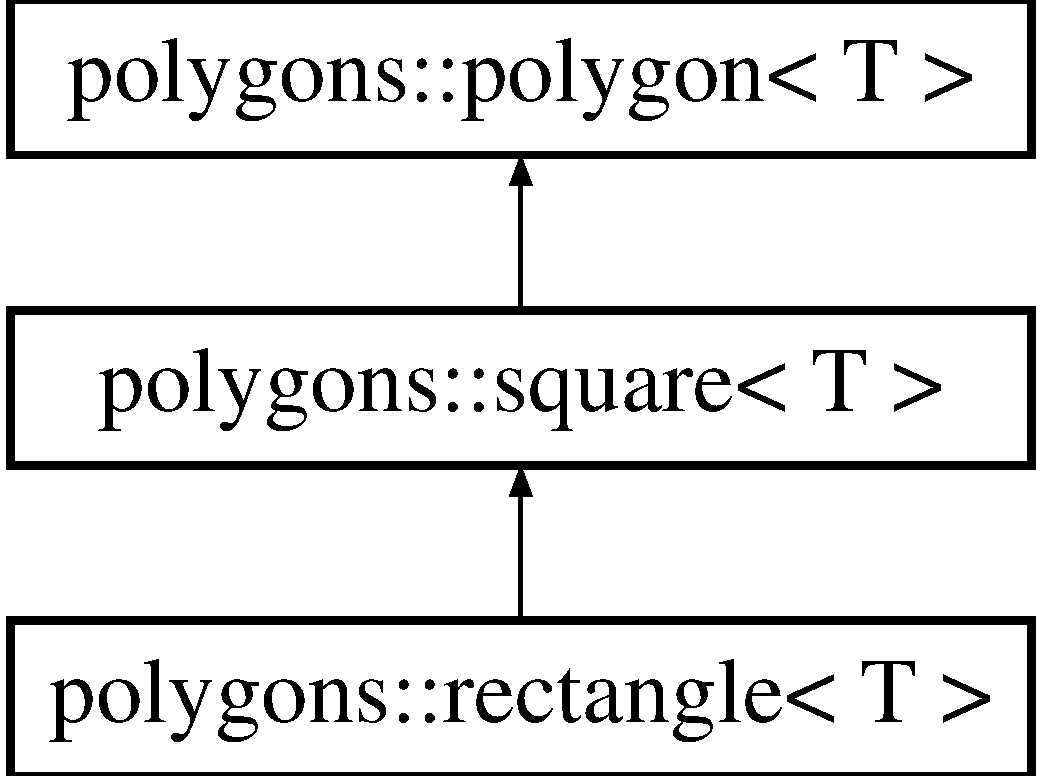
\includegraphics[height=3.000000cm]{classpolygons_1_1rectangle}
\end{center}
\end{figure}
\subsection*{Public Member Functions}
\begin{DoxyCompactItemize}
\item 
\hypertarget{classpolygons_1_1rectangle_a41ebba3925afeb3bf73b836c41089bb2}{{\bfseries rectangle} (T p\-\_\-x, T p\-\_\-y, T p\-\_\-\-W, T p\-\_\-\-H)}\label{classpolygons_1_1rectangle_a41ebba3925afeb3bf73b836c41089bb2}

\item 
\hypertarget{classpolygons_1_1rectangle_a92e64e9f8e05bfd15fdfd2e24be93ae9}{string {\bfseries type} ()}\label{classpolygons_1_1rectangle_a92e64e9f8e05bfd15fdfd2e24be93ae9}

\end{DoxyCompactItemize}
\subsection*{Additional Inherited Members}


The documentation for this class was generated from the following file\-:\begin{DoxyCompactItemize}
\item 
polygon.\-h\end{DoxyCompactItemize}

\hypertarget{classpolygons_1_1square}{\section{polygons\-:\-:square$<$ T $>$ Class Template Reference}
\label{classpolygons_1_1square}\index{polygons\-::square$<$ T $>$@{polygons\-::square$<$ T $>$}}
}
Inheritance diagram for polygons\-:\-:square$<$ T $>$\-:\begin{figure}[H]
\begin{center}
\leavevmode
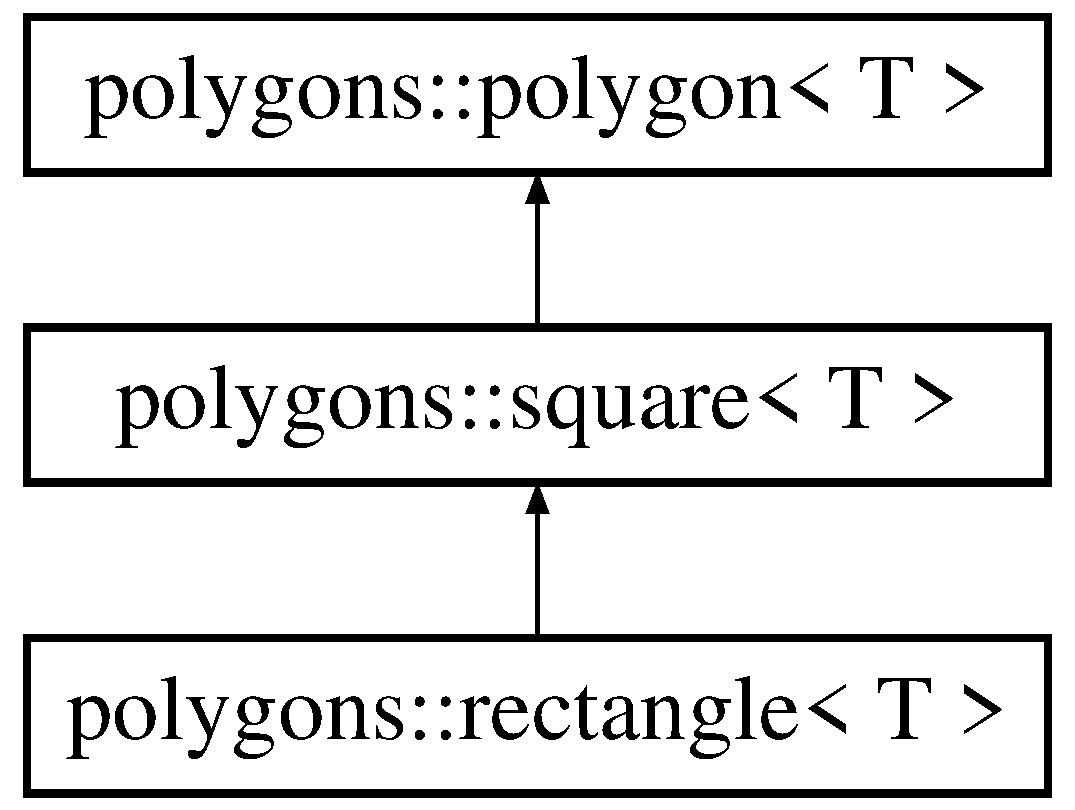
\includegraphics[height=3.000000cm]{classpolygons_1_1square}
\end{center}
\end{figure}
\subsection*{Public Member Functions}
\begin{DoxyCompactItemize}
\item 
\hypertarget{classpolygons_1_1square_a33bfdb2f23cbe2ad48fe67a2c1bc94ae}{{\bfseries square} (T p\-\_\-x, T p\-\_\-y, T p\-\_\-\-L)}\label{classpolygons_1_1square_a33bfdb2f23cbe2ad48fe67a2c1bc94ae}

\item 
\hypertarget{classpolygons_1_1square_ab39ca97ab49022aba1c4773de116fc50}{string {\bfseries type} ()}\label{classpolygons_1_1square_ab39ca97ab49022aba1c4773de116fc50}

\end{DoxyCompactItemize}
\subsection*{Additional Inherited Members}


The documentation for this class was generated from the following file\-:\begin{DoxyCompactItemize}
\item 
polygon.\-h\end{DoxyCompactItemize}

\hypertarget{classpolygons_1_1vertex}{\section{polygons\-:\-:vertex$<$ T $>$ Class Template Reference}
\label{classpolygons_1_1vertex}\index{polygons\-::vertex$<$ T $>$@{polygons\-::vertex$<$ T $>$}}
}
\subsection*{Public Member Functions}
\begin{DoxyCompactItemize}
\item 
\hypertarget{classpolygons_1_1vertex_a084c44b137174a94324e5cc21c132090}{{\bfseries vertex} (T p\-\_\-x1, T p\-\_\-x2, T p\-\_\-x3)}\label{classpolygons_1_1vertex_a084c44b137174a94324e5cc21c132090}

\item 
\hypertarget{classpolygons_1_1vertex_ac83cc341b484203c928f6e63831aff4f}{{\bfseries vertex} (const \hyperlink{classpolygons_1_1vertex}{vertex}$<$ T $>$ \&)}\label{classpolygons_1_1vertex_ac83cc341b484203c928f6e63831aff4f}

\item 
\hypertarget{classpolygons_1_1vertex_ac8149193ad9abf7e7848517c18e51a48}{\hyperlink{classpolygons_1_1vertex}{vertex}$<$ T $>$ \& {\bfseries operator=} (const \hyperlink{classpolygons_1_1vertex}{vertex}$<$ T $>$ \&)}\label{classpolygons_1_1vertex_ac8149193ad9abf7e7848517c18e51a48}

\item 
\hypertarget{classpolygons_1_1vertex_ace58802bc7034a44912bb5e9e2237d8f}{T {\bfseries x} ()}\label{classpolygons_1_1vertex_ace58802bc7034a44912bb5e9e2237d8f}

\item 
\hypertarget{classpolygons_1_1vertex_aef04f860e36ffa6eb0850a7300fa0595}{T {\bfseries y} ()}\label{classpolygons_1_1vertex_aef04f860e36ffa6eb0850a7300fa0595}

\item 
\hypertarget{classpolygons_1_1vertex_a9df987b209969024e8e0a06c084337a0}{T {\bfseries z} ()}\label{classpolygons_1_1vertex_a9df987b209969024e8e0a06c084337a0}

\item 
\hypertarget{classpolygons_1_1vertex_aabddd9c7117d9bf99165ddc421ee8a3e}{T {\bfseries x} (int p\-\_\-i)}\label{classpolygons_1_1vertex_aabddd9c7117d9bf99165ddc421ee8a3e}

\item 
\hypertarget{classpolygons_1_1vertex_a2fb39cd8b338d23851c04d087c151825}{void {\bfseries x} (T p\-\_\-x)}\label{classpolygons_1_1vertex_a2fb39cd8b338d23851c04d087c151825}

\item 
\hypertarget{classpolygons_1_1vertex_aaee907890acfc192b3bdccdf1f2a49fd}{void {\bfseries y} (T p\-\_\-y)}\label{classpolygons_1_1vertex_aaee907890acfc192b3bdccdf1f2a49fd}

\item 
\hypertarget{classpolygons_1_1vertex_a7f5cdb953ab958f8205d0613198927d5}{void {\bfseries z} (T p\-\_\-z)}\label{classpolygons_1_1vertex_a7f5cdb953ab958f8205d0613198927d5}

\item 
\hypertarget{classpolygons_1_1vertex_a580ba47cb1310c14fb627cfe586caa1f}{void {\bfseries pos} (T p\-\_\-x, T p\-\_\-y, T p\-\_\-z)}\label{classpolygons_1_1vertex_a580ba47cb1310c14fb627cfe586caa1f}

\item 
\hypertarget{classpolygons_1_1vertex_a734a367601a84d9328be94d0d4a3b74a}{void {\bfseries translate} (T p\-\_\-x, T p\-\_\-y, T p\-\_\-z)}\label{classpolygons_1_1vertex_a734a367601a84d9328be94d0d4a3b74a}

\item 
\hypertarget{classpolygons_1_1vertex_a181e0714703ed81ed70cdb512f55dfaf}{void {\bfseries rotate\-X} (T p\-\_\-theta)}\label{classpolygons_1_1vertex_a181e0714703ed81ed70cdb512f55dfaf}

\item 
\hypertarget{classpolygons_1_1vertex_ab0b42c9271695811f90002290837c528}{void {\bfseries rotate\-Y} (T p\-\_\-theta)}\label{classpolygons_1_1vertex_ab0b42c9271695811f90002290837c528}

\item 
\hypertarget{classpolygons_1_1vertex_afd0e8a9c607babecc23ec304cfb300bf}{void {\bfseries rotate\-Z} (T p\-\_\-theta)}\label{classpolygons_1_1vertex_afd0e8a9c607babecc23ec304cfb300bf}

\item 
\hypertarget{classpolygons_1_1vertex_a61d7eec7a044510d32adf5af34a3fc60}{void {\bfseries rotate} (T p\-\_\-x1, T p\-\_\-y1, T p\-\_\-z1, T p\-\_\-x2, T p\-\_\-y2, T p\-\_\-z2, T p\-\_\-theta)}\label{classpolygons_1_1vertex_a61d7eec7a044510d32adf5af34a3fc60}

\item 
\hypertarget{classpolygons_1_1vertex_a61930a82c90b43714d413a5af1f1c504}{void {\bfseries scale} (T p\-\_\-x, T p\-\_\-y, T p\-\_\-z, T p\-\_\-fx, T p\-\_\-fy, T p\-\_\-fz)}\label{classpolygons_1_1vertex_a61930a82c90b43714d413a5af1f1c504}

\end{DoxyCompactItemize}
\subsection*{Protected Attributes}
\begin{DoxyCompactItemize}
\item 
\hypertarget{classpolygons_1_1vertex_afa8a8def08c6d6894e21a945845b165e}{T {\bfseries m\-\_\-x} \mbox{[}3\mbox{]}}\label{classpolygons_1_1vertex_afa8a8def08c6d6894e21a945845b165e}

\end{DoxyCompactItemize}
\subsection*{Friends}
\begin{DoxyCompactItemize}
\item 
\hypertarget{classpolygons_1_1vertex_af4bb2e5e1c59f13862d734823e541911}{ostream \& {\bfseries operator$<$$<$} (ostream \&p\-\_\-out\-Stream, \hyperlink{classpolygons_1_1vertex}{vertex}$<$ T $>$ const \&p\-\_\-vtx)}\label{classpolygons_1_1vertex_af4bb2e5e1c59f13862d734823e541911}

\end{DoxyCompactItemize}


The documentation for this class was generated from the following file\-:\begin{DoxyCompactItemize}
\item 
vertex.\-h\end{DoxyCompactItemize}

%--- End generated contents ---

% Index
\newpage
\phantomsection
\addcontentsline{toc}{chapter}{Index}
\printindex

\end{document}
